% Anhang
%

\chapter{Profiling}

For the profiling an own implementation is used based on wall clock timings.
An own implementation is
chosen to have full control about the disk and memory access of the profiler.
So io interruptions caused by the profiler are avoided.

Used code to get current timestamp:

\begin{lstlisting}
enum
{
	MICROSEC = (timeunit_t)1,
	MILLISEC = MICROSEC * 1000,
	SECONDS  = MILLISEC * 1000,
};

uint64_t get_timestamp ()
{
    struct timeval now;
    gettimeofday (&now, (struct timezone*)0);
    return  (uint64_t) now.tv_usec + 
            (uint64_t) now.tv_sec * SECONDS;
}
\end{lstlisting}

TraceLogger class handles the the measurements.
It generates buffers in the initialization and writes the measurements to file in the destruction.
For instrument a specific block or function in the algorithm \emph{start} and \emph{stop} function
\begin{lstlisting}
tracelogger.begin(0,"sort");
sort_function();
tracelogger.end(0,"sort");
\end{lstlisting}

The measured timings are written to an csv file, which has e.g. the following content:
\begin{lstlisting}
0;0;run;0;3793;116429658;
0;0;loadSynapses;0;2622330;4432049;
0;0;sort;0;4519751;5770458;
0;0;communicate;0;5770465;6366961;
\end{lstlisting}


Each row specifies one measurement. The columns contain the rank number, thread number, function name,
iteration number, start time and finish time respectively.

To get an overview the numbers are plotted in a raster plot.

\begin{figure}[ht!]
\centering
\includegraphics[scale=0.4]{pictures/1per300_tracefile_connect.png}
\caption{Visualized trace file}
\end{figure}

\chapter{Measure memory consumption}

\begin{lstlisting}


#include <stdio.h>
#include <spi/include/kernel/memory.h>

int getMemoryInformation(..)
{
  uint64_t shared, persist, heapavail, stackavail, stack, heap, guard, mmap;

  Kernel_GetMemorySize(KERNEL_MEMSIZE_SHARED, &shared);
  Kernel_GetMemorySize(KERNEL_MEMSIZE_PERSIST, &persist);
  Kernel_GetMemorySize(KERNEL_MEMSIZE_HEAPAVAIL, &heapavail);
  Kernel_GetMemorySize(KERNEL_MEMSIZE_STACKAVAIL, &stackavail);
  Kernel_GetMemorySize(KERNEL_MEMSIZE_STACK, &stack);
  Kernel_GetMemorySize(KERNEL_MEMSIZE_HEAP, &heap);
  Kernel_GetMemorySize(KERNEL_MEMSIZE_GUARD, &guard);
  Kernel_GetMemorySize(KERNEL_MEMSIZE_MMAP, &mmap);

  ..
}

\end{lstlisting}

\chapter{Mouse brain model standard use-case}
\label{ambmusecase}
In the thesis one virtual experiment is applied mostly to the mouse brain model inside of NEST.
The neurons, which are related to the left whiskers, are stimulated.
Therefore the neuron HDF5 file contain a subnet dataset which contain a zero
for all neurons except of the related neurons. The related neurons have the entry 1.
A constant input current of 2500pA is set for these neurons with the \emph{SLI} function \emph{set\_status}.
A multimeter and spikedetector observes all neurons.
The circuit is simulated for 1000ms.

\chapter{HDF5 file of voxel list of long range generation}
\label{file:voxelinfo}
The list of processed voxels which is generated by the long range generation can be exported and imported
by the generation program. Therefore manipulation and debugging of the long range connections generation should be
simplified. The HDF5 file can be visualized and modified easily with Python. Further use-cases are 
splitting the generation in several files. Thus smaller synapse files can be generated.

\begin{figure}[ht!]
\centering
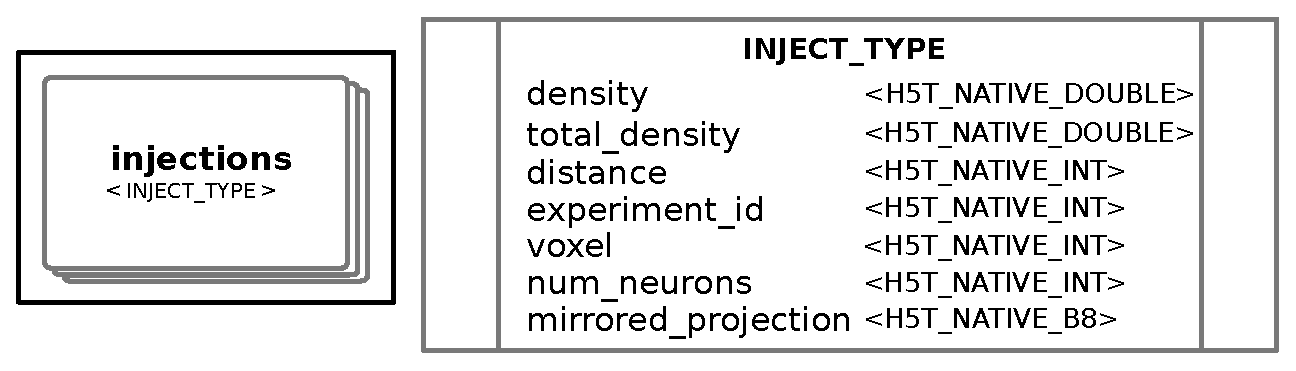
\includegraphics[scale=0.6]{pictures/hdf5_voxel_format.eps}
\caption{HDF5 voxel information file structure}
\end{figure}

Each voxel entry contains the following entries: density of the injection for the given voxel (\emph{density}),
total injection of the selected experiment (\emph{total\_density}),
interpolated quality (\emph{distance} of nearest neighbour algorithm, zero if no interpolation needed for the voxel.),
reference to the selected experiment (\emph{experiment\_id}),
voxel id (\emph{voxel}),
number of neurons inside of voxel (\emph{num\_neurons}) and
a logical value, if the voxel was mirrored (\emph{mirrored\_projection}).



\chapter{Tools}

\section{h5py}
\label{sec:h5py}
The h5py package is a Pythonic interface to the HDF5 binary data format.
It lets you store huge amounts of numerical data, and easily manipulate that data from NumPy. For example, you can slice into multi-terabyte datasets stored on disk, as if they were real NumPy arrays. Thousands of datasets can be stored in a single file, categorized and tagged however you want.
H5py uses straightforward NumPy and Python metaphors, like dictionary and NumPy array syntax. For example, you can iterate over datasets in a file, or check out the .shape or .dtype attributes of datasets. \cite{h5py}
\section{numpy}
\label{sec:numpy}
NumPy is an extension to the Python programming language, adding support for large, multi-dimensional arrays and matrices, along with a large library of high-level mathematical functions to operate on these arrays. The ancestor of NumPy, Numeric, was originally created by Jim Hugunin with contributions from several other developers. In 2005, Travis Oliphant created NumPy by incorporating features of the competing Numarray into Numeric, with extensive modifications. NumPy is open source and has many contributors. \cite{numpy}
\section{matplotlib}
\label{sec:matplotlib}
matplotlib is a plotting library for the Python programming language and its numerical mathematics extension NumPy. It provides an object-oriented API for embedding plots into applications using general-purpose GUI toolkits like wxPython, Qt, or GTK+. There is also a procedural "pylab" interface based on a state machine (like OpenGL), designed to closely resemble that of MATLAB. SciPy makes use of matplotlib.
matplotlib was originally written by John D. Hunter, has an active development community,[1] and is distributed under a BSD-style license. \cite{matplotlib}
\section{MetaImage}
\label{sec:MetaImage}
MetaImage is the text-based tagged file format for medical images that resulted. \cite{metaimage}
It is based on a descriptive ascii file and a binary file.
The ascii file contains all meta data of the data stored inside the binary file.

For the my use case a 3d voxelized dataset is stored inside the MetaImage format.
The ascii files contains information about the datatype, dimensions and byte order.
Thus a 1d projection of the 3d voxelized dataset inside the binary file can be read in the correct order.

\section{Voxelize}
\label{sec:voxelize}
Voxelize is a library of Livre handling the voxelisation of different data sources (surface meshes, BBP morphologies, local-field potentials, etc) through the use of plugins.\cite{livre}
It can be used seperatly to generate MetaImage files containing geometrical placements of neuron clouds (given the the specified neuron file format).
\section{Livre}
\label{sec:livre}
Livre (Large-scale Interactive Volume Rendering Engine) is an out-of-core, multi-node, multi-gpu, OpenGL volume rendering engine to visualise large volumetric data sets.
It provides the following major features to facilitate rendering of large volumetric data sets \cite{livre}:
\begin{itemize}
    \item Visualisation of pre-processed UVF format (source code) volume data sets.
    \item Real-time voxelisation of different data sources (surface meshes, BBP morphologies, local-field potentials, etc) through the use of plugins.
    \item Multi-node, multi-gpu rendering (Currently only sort-first rendering)
\end{itemize}
\section{Paraview}
\label{sec:paraview}
ParaView is an open-source, multi-platform application designed to visualize data sets of varying sizes from small to very large. The goals of the ParaView project include developing an open-source, multi-platform visualization application that supports distributed computational models to process large data sets. It has an open, flexible, and intuitive user interface. Furthermore, ParaView is built on an extensible architecture based on open standards. ParaView runs on distributed and shared memory parallel as well as single processor systems and has been succesfully tested on Windows, Linux, Mac OS X, IBM Blue Gene, Cray XT3 and various Unix workstations and clusters. Under the hood, ParaView uses the Visualization Toolkit as the data processing and rendering engine and has a user interface written using the Qt cross-platform application framework. \cite{paraview}

